\documentclass[tikz]{standalone}
\usetikzlibrary{arrows.meta,positioning,calc}
\begin{document}
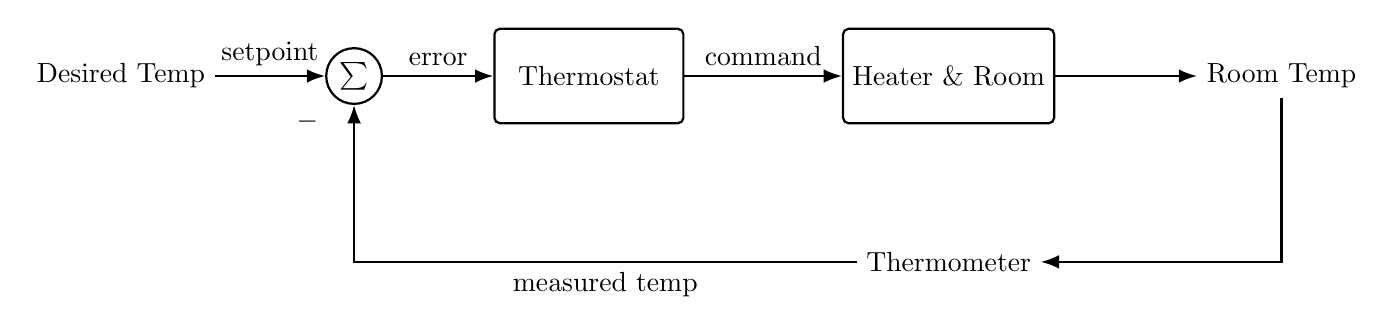
\begin{tikzpicture}[>=LaTeX,block/.style={draw,minimum width=2.4cm,minimum height=1.2cm,rounded corners=2pt,thick},sum/.style={draw,circle,inner sep=2pt,thick},node distance=1.6cm]
  \node (ref) {Desired Temp};
  \node[sum,right=1.4cm of ref] (sum) {$\sum$};
  \node[block,right=1.4cm of sum] (ctrl) {Thermostat};
  \node[block,right=2cm of ctrl] (plant) {Heater \& Room};
  \node[right=1.8cm of plant] (out) {Room Temp};
  \node[below=1.5cm of plant] (meas) {Thermometer};
  \draw[->,thick] (ref) -- node[midway,above]{setpoint} (sum);
  \draw[->,thick] (sum) -- node[midway,above]{error} (ctrl);
  \draw[->,thick] (ctrl) -- node[midway,above]{command} (plant);
  \draw[->,thick] (plant) -- (out);
  \draw[->,thick] (out) |- (meas);
  \draw[->,thick] (meas) -| node[pos=0.25,below]{measured temp} (sum);
  \node[below left=0.1cm of sum] {$-$};
\end{tikzpicture}
\end{document}
